

\tikzset{every picture/.style={line width=0.75pt}} %set default line width to 0.75pt        

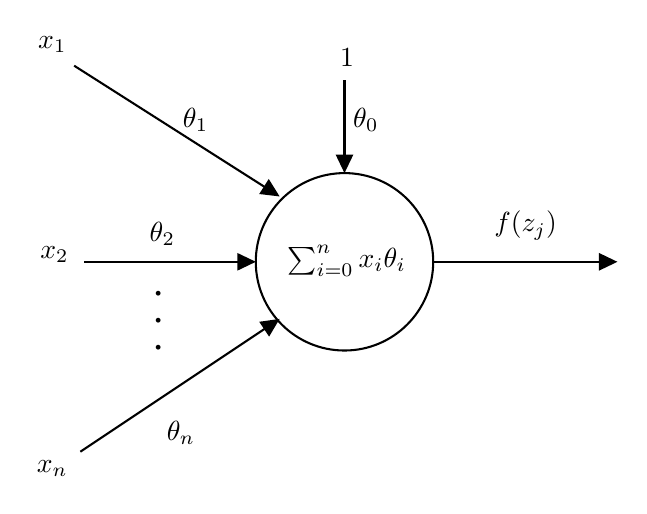
\begin{tikzpicture}[x=0.75pt,y=0.75pt,yscale=-1,xscale=1]
%uncomment if require: \path (0,300); %set diagram left start at 0, and has height of 300

%Straight Lines [id:da680897344066558] 
\draw    (223.5,117.49) -- (310.25,117.49) ;
\draw [shift={(312.25,117.49)}, rotate = 180] [fill={rgb, 255:red, 0; green, 0; blue, 0 }  ][line width=0.75]  [draw opacity=0] (8.93,-4.29) -- (0,0) -- (8.93,4.29) -- cycle    ;

%Shape: Circle [id:dp9729890208928396] 
\draw   (138.02,117.49) .. controls (138.02,93.89) and (157.15,74.75) .. (180.76,74.75) .. controls (204.36,74.75) and (223.5,93.89) .. (223.5,117.49) .. controls (223.5,141.1) and (204.36,160.23) .. (180.76,160.23) .. controls (157.15,160.23) and (138.02,141.1) .. (138.02,117.49) -- cycle ;
%Straight Lines [id:da595997026089699] 
\draw    (50.5,23) -- (147.81,84.93) ;
\draw [shift={(149.5,86)}, rotate = 212.47] [fill={rgb, 255:red, 0; green, 0; blue, 0 }  ][line width=0.75]  [draw opacity=0] (8.93,-4.29) -- (0,0) -- (8.93,4.29) -- cycle    ;

%Straight Lines [id:da17014503403275416] 
\draw    (55.49,117.49) -- (136.02,117.49) ;
\draw [shift={(138.02,117.49)}, rotate = 540] [fill={rgb, 255:red, 0; green, 0; blue, 0 }  ][line width=0.75]  [draw opacity=0] (8.93,-4.29) -- (0,0) -- (8.93,4.29) -- cycle    ;

%Straight Lines [id:da3776987769018221] 
\draw    (53.5,209) -- (147.84,146.11) ;
\draw [shift={(149.5,145)}, rotate = 506.31] [fill={rgb, 255:red, 0; green, 0; blue, 0 }  ][line width=0.75]  [draw opacity=0] (8.93,-4.29) -- (0,0) -- (8.93,4.29) -- cycle    ;

%Straight Lines [id:da22738163646288978] 
\draw    (180.76,30.12) -- (180.76,72.75) ;
\draw [shift={(180.76,74.75)}, rotate = 270] [fill={rgb, 255:red, 0; green, 0; blue, 0 }  ][line width=0.75]  [draw opacity=0] (8.93,-4.29) -- (0,0) -- (8.93,4.29) -- cycle    ;


% Text Node
\draw (184,117) node   {$\sum ^{n}_{i=0} x_{i} \theta _{i} \ $};
% Text Node
\draw (91,146) node [rotate=-90] [align=left] {\textbf{{\large . . .}}};
% Text Node
\draw (40,13) node   {$x_{1}$};
% Text Node
\draw (41,114) node   {$x_{2}$};
% Text Node
\draw (40,217) node   {$x_{n}$};
% Text Node
\draw (182,19) node   {$1$};
% Text Node
\draw (109,49) node   {$\theta _{1}$};
% Text Node
\draw (93,104) node   {$\theta _{2}$};
% Text Node
\draw (102,200) node   {$\theta _{n}$};
% Text Node
\draw (268,100) node   {$f( z_{j})$};
% Text Node
\draw (191,49) node   {$\theta _{0}$};


\end{tikzpicture}
